% !TeX root = ../thuthesis-example.tex

\chapter{测试驱动开发的设计与实现}
\label{chap:tdd}

测试驱动开发(Test-Driven Development, TDD)是一种软件开发方法论,核心在于先编写测试代码再实现功能代码。这种"测试先行"范式要求开发者首先明确定义预期行为与结果,随后实现满足测试条件的功能代码。TDD遵循"红-绿-重构"循环:编写一个失败的测试(红),实现最小可行代码使测试通过(绿),最后改进代码结构与设计(重构)。

bolt.SE的测试模块是对TDD理念的工程化实现,使开发者能创建、管理测试用例,并引导大语言模型(LLM)生成满足这些测试要求的代码。本章分析TDD概念、方法论价值及bolt.SE的测试功能技术实现。

\section{测试驱动开发的概念与意义}

\subsection{TDD在软件工程中的优势}
测试驱动开发为软件工程带来了以下关键优势:

\begin{enumerate}
  \item \textbf{设计优先}:TDD驱使开发者在实现前思考接口设计与行为规范,促成更清晰的模块化结构。
  
  \item \textbf{快速反馈}:代码更改后立即运行测试,提供即时反馈,使问题在早期就能被发现。
  
  \item \textbf{回归保障}:完整测试套件构成代码重构与功能迭代的安全网,减少变更引入缺陷的风险。
  
  \item \textbf{活文档效应}:测试代码准确记录系统预期行为,形成自动与代码同步更新的技术文档。
  
  \item \textbf{聚焦实现}:明确的测试目标减少了开发过程中的决策疲劳,避免过度工程和不必要的复杂性。
\end{enumerate}

在bolt.SE这类开发平台中,结构化测试定义与自动化执行进一步增强了这些优势,优化开发流程并提高代码质量。

\subsection{TDD对LLM驱动开发的价值}
在大型语言模型驱动的软件开发中,测试驱动方法具有特殊价值\cite{Mathews2024}:

\begin{enumerate}
  \item \textbf{需求形式化}:测试用例为LLM提供结构化需求表达,降低需求理解的歧义性。
  
  \item \textbf{约束生成空间}:测试明确定义预期行为,为LLM提供具体目标,限定代码生成的解空间。
  
  \item \textbf{控制生成质量}:严格的测试约束降低LLM生成错误或不切实际代码的风险,强制输出需符合验证逻辑。
  
  \item \textbf{验证生成结果}:测试提供客观验证机制,确保LLM生成的代码能正确运行而非仅表面合理。
  
  \item \textbf{支持持续优化}:测试结果为LLM提供结构化反馈,引导其精确改进代码缺陷。
\end{enumerate}

bolt.SE将测试代码集成至对话上下文,实现了LLM与测试用例的协同工作模式。这种方法既保留了LLM的生成灵活性,又引入了软件工程的严谨验证机制。

\section{Jest测试框架与TDD实践}

Jest是Facebook开发的JavaScript测试框架,以简洁易用著称,已成为前端测试领域的主流选择\cite{Jest2023}。bolt.SE采用Jest作为测试功能核心框架,并针对TDD工作流进行了优化。

\subsection{Jest测试框架概述}

Jest提供了全面的测试工具集,具备以下核心特性:

\begin{enumerate}
  \item \textbf{零配置测试环境}:内置断言库、测试运行器和模拟工具,最小化配置开销。
  
  \item \textbf{声明式测试API}:通过\texttt{describe}、\texttt{it}/\texttt{test}和\texttt{expect}等函数构建清晰、易读的测试结构。
  
  \item \textbf{快照测试机制}:支持UI组件和数据结构的版本比对,简化回归测试流程。
  
  \item \textbf{多样化断言器}:提供丰富的匹配器,适应不同测试场景需求。
  
  \item \textbf{并行执行能力}:默认并行运行测试,优化执行效率。
  
  \item \textbf{覆盖率分析}:内置代码覆盖率统计与可视化报告。
\end{enumerate}

在bolt.SE中,Jest测试通常采用如下结构:

\begin{minted}{javascript}
// 测试套件
describe('Calculator', () => {
  // 测试用例
  test('adds 1 + 2 to equal 3', () => {
    expect(add(1, 2)).toBe(3);
  });
  
  test('subtracts 5 - 2 to equal 3', () => {
    expect(subtract(5, 2)).toBe(3);
  });
});
\end{minted}

bolt.SE测试模块解析此结构,提取测试套件与用例信息,并将其转化为LLM可理解的约束条件。

\subsection{TDD工作流程}

bolt.SE环境中的TDD工作流程整合了传统测试驱动与AI辅助开发的优势:

\begin{enumerate}
  \item \textbf{测试定义}:开发者在专用编辑器中创建测试代码,明确定义功能行为规范。
  
  \item \textbf{结构提取}:系统自动解析测试代码,构建测试套件和用例的树形结构表示。
  
  \item \textbf{上下文注入}:新建对话时,系统将测试代码作为上下文信息传递给LLM。
  
  \item \textbf{代码生成}:LLM基于测试约束理解需求,生成满足测试条件的实现代码。
  
  \item \textbf{测试验证}:开发者执行测试,验证生成代码是否符合预期行为。
  
  \item \textbf{迭代更新}:根据测试结果调整代码或测试用例,形成开发迭代环。
\end{enumerate}

此工作流程将TDD的规范性与AI生成的高效性结合,实现了更精确、高效的开发模式。

\section{bolt.SE测试功能技术实现}

bolt.SE将TDD原则融入系统架构,通过模块化设计实现了测试驱动的AI辅助开发流程。本节分析其技术实现,包括架构设计、核心组件和功能机制。

\begin{figure}[htbp]
  \centering
  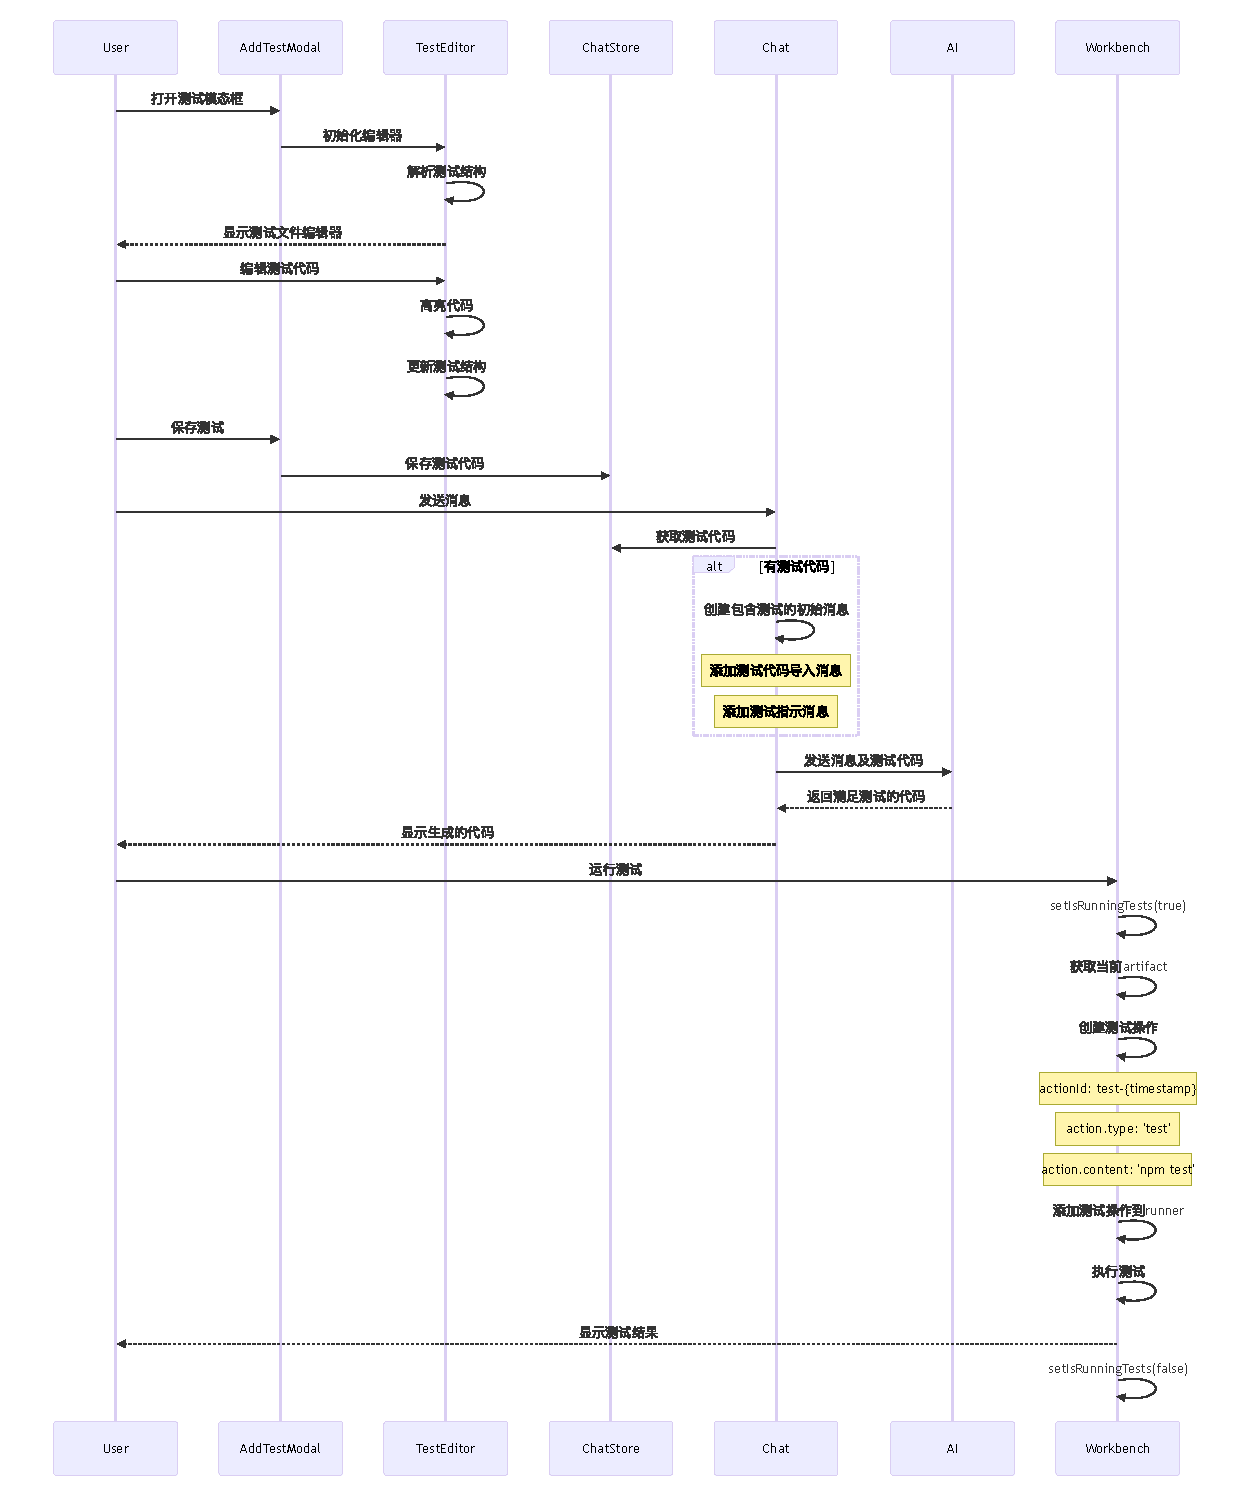
\includegraphics[width=\textwidth]{figures/bolt_test_sequence.pdf}
  \caption{测试功能流程图:展示用户测试定义、使用及验证的完整流程与跨组件信息传递机制}
  \label{fig:test_sequence}
\end{figure}

\subsection{架构设计与模块构成}

bolt.SE测试系统采用组件化架构,主要包含以下核心模块:

\begin{enumerate}
  \item \textbf{用户界面层}:
    \begin{itemize}
      \item \texttt{AddTestModal}:测试管理的主入口,支持测试创建与编辑
      \item \texttt{TestEditor}:代码编辑器组件,提供语法高亮与结构可视化
      \item \texttt{TestStructure}:测试树渲染组件,展示测试套件与用例的层次关系
    \end{itemize}
  
  \item \textbf{数据处理层}:
    \begin{itemize}
      \item \texttt{chatStore}:管理当前会话的测试代码集合
      \item \texttt{IndexedDB}:持久化存储测试定义,支持跨会话访问
    \end{itemize}
  
  \item \textbf{测试执行层}:
    \begin{itemize}
      \item \texttt{Workbench}:提供测试运行环境与命令执行
      \item \texttt{ActionRunner}:负责测试调度与结果采集
    \end{itemize}
  
  \item \textbf{AI交互层}:处理测试代码与LLM的信息交换与指令生成
\end{enumerate}

如图\ref{fig:test_sequence}所示,测试流程分为定义、使用和验证三个主要阶段,构成完整的测试生命周期管理。

bolt.SE定义了结构化的测试数据模型,如图\ref{fig:test_class}所示:

\begin{figure}[htbp]
  \centering
  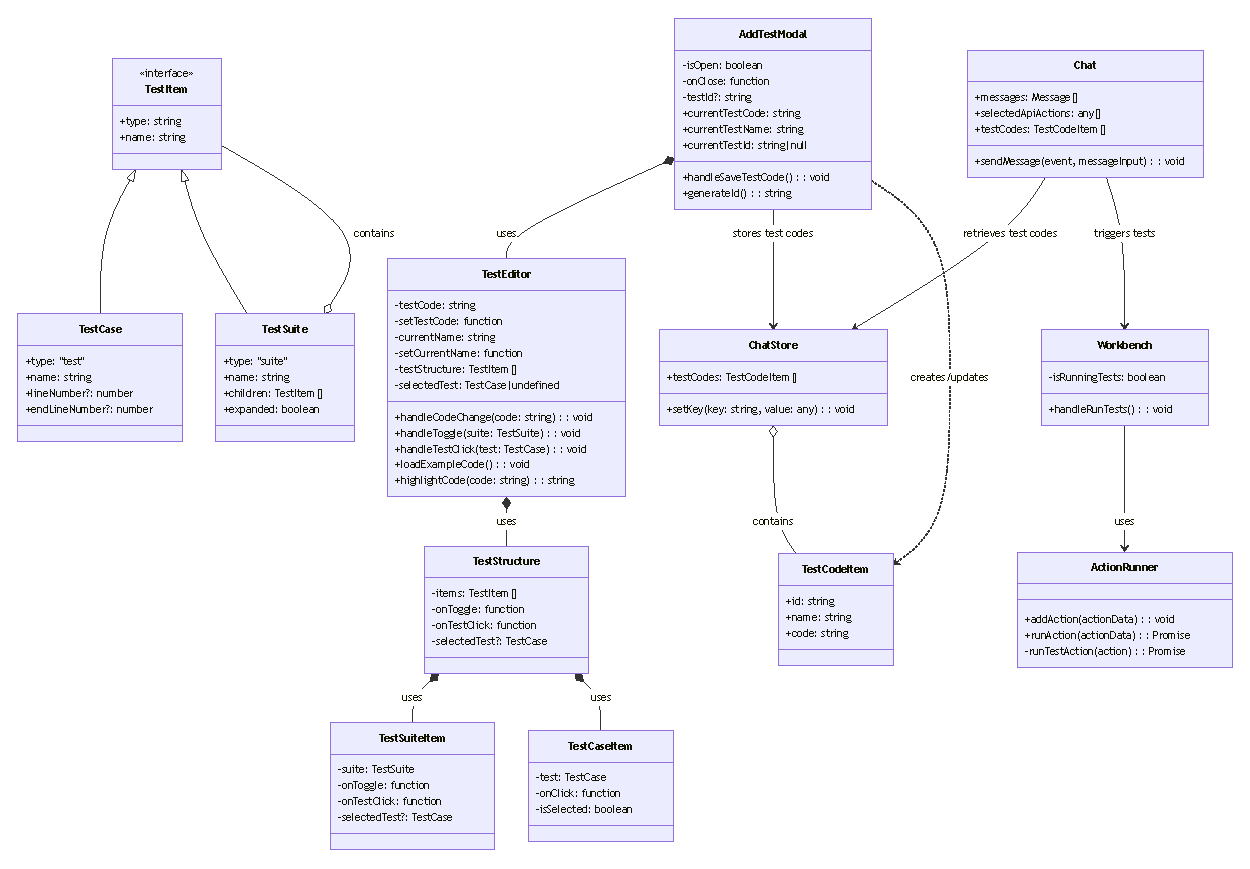
\includegraphics[width=\textwidth]{figures/bolt_test_class.pdf}
  \caption{测试数据模型类图:描述测试定义的核心数据结构及关系,包含测试代码项、测试用例与测试套件的层次组织}
  \label{fig:test_class}
\end{figure}

核心数据结构包括:

\begin{enumerate}
  \item \textbf{TestCodeItem}:测试文件实体,包含唯一标识符、名称与代码内容。
  
  \item \textbf{TestItem}:测试项基础接口,定义共用的类型与名称属性。
  
  \item \textbf{TestCase}:具体测试用例,标识类型为"test",记录代码位置信息。
  
  \item \textbf{TestSuite}:测试套件,标识类型为"suite",包含子测试项集合与展开状态。
\end{enumerate}

系统实现了以下关键功能:

\begin{enumerate}
  \item \textbf{测试解析}:解析Jest测试代码,提取测试结构并构建层次化表示。
  
  \item \textbf{结构编辑}:提供专用编辑界面,支持测试代码创建与修改。
  
  \item \textbf{上下文集成}:将测试转换为文件操作指令,注入对话上下文。
  
  \item \textbf{执行验证}:通过Workbench提供测试执行环境,验证代码符合性。
  
  \item \textbf{结果反馈}:收集并可视化测试执行结果,支持问题定位与修复。
\end{enumerate}

\subsection{测试解析与可视化机制}

bolt.SE实现了高效的测试代码解析与可视化机制:

\begin{enumerate}
  \item \textbf{语法分析}:采用正则表达式识别\texttt{describe}和\texttt{it}/\texttt{test}函数调用,提取测试结构。
  
  \item \textbf{树形建模}:基于代码的语法嵌套关系,构建测试的层次结构模型。
  
  \item \textbf{位置映射}:记录每个测试用例在源码中的行号范围,支持双向定位。
  
  \item \textbf{交互式视图}:提供可折叠的测试树结构,支持灵活导航与管理。
  
  \item \textbf{同步高亮}:点击测试项时自动定位并高亮相应代码区域。
\end{enumerate}

这些机制显著提升了测试代码的可读性与可管理性,简化了复杂测试套件的维护工作。

\subsection{测试与LLM协同机制}

bolt.SE创新地实现了测试与LLM的协同工作机制:

\begin{enumerate}
  \item \textbf{上下文嵌入}:启动对话时,系统将测试代码转换为结构化指令注入对话上下文。
  
  \item \textbf{行为引导}:生成专门的指导信息,明确告知LLM需基于测试生成代码及相关环境配置。
  
  \item \textbf{环境配置}:指导LLM添加必要依赖和测试脚本,自动构建测试环境。
  
  \item \textbf{验证机制}:要求在功能代码完成后立即执行测试,确保符合预期行为。
  
  \item \textbf{修复循环}:测试失败时将错误信息回传给LLM,引导其进行针对性修复。
\end{enumerate}

这种协同机制使LLM能够理解并遵循TDD原则,在严格约束下生成高质量代码。

\section{实例应用场景}
\label{sec:tdd-example}

本节通过JavaScript计算器的完整开发流程,展示bolt.SE中基于"红–绿–重构"循环的测试驱动开发过程及LLM参与的自动修复机制。

\subsection{插入Jest测试代码与需求声明}

\begin{figure}[htbp]
  \centering
  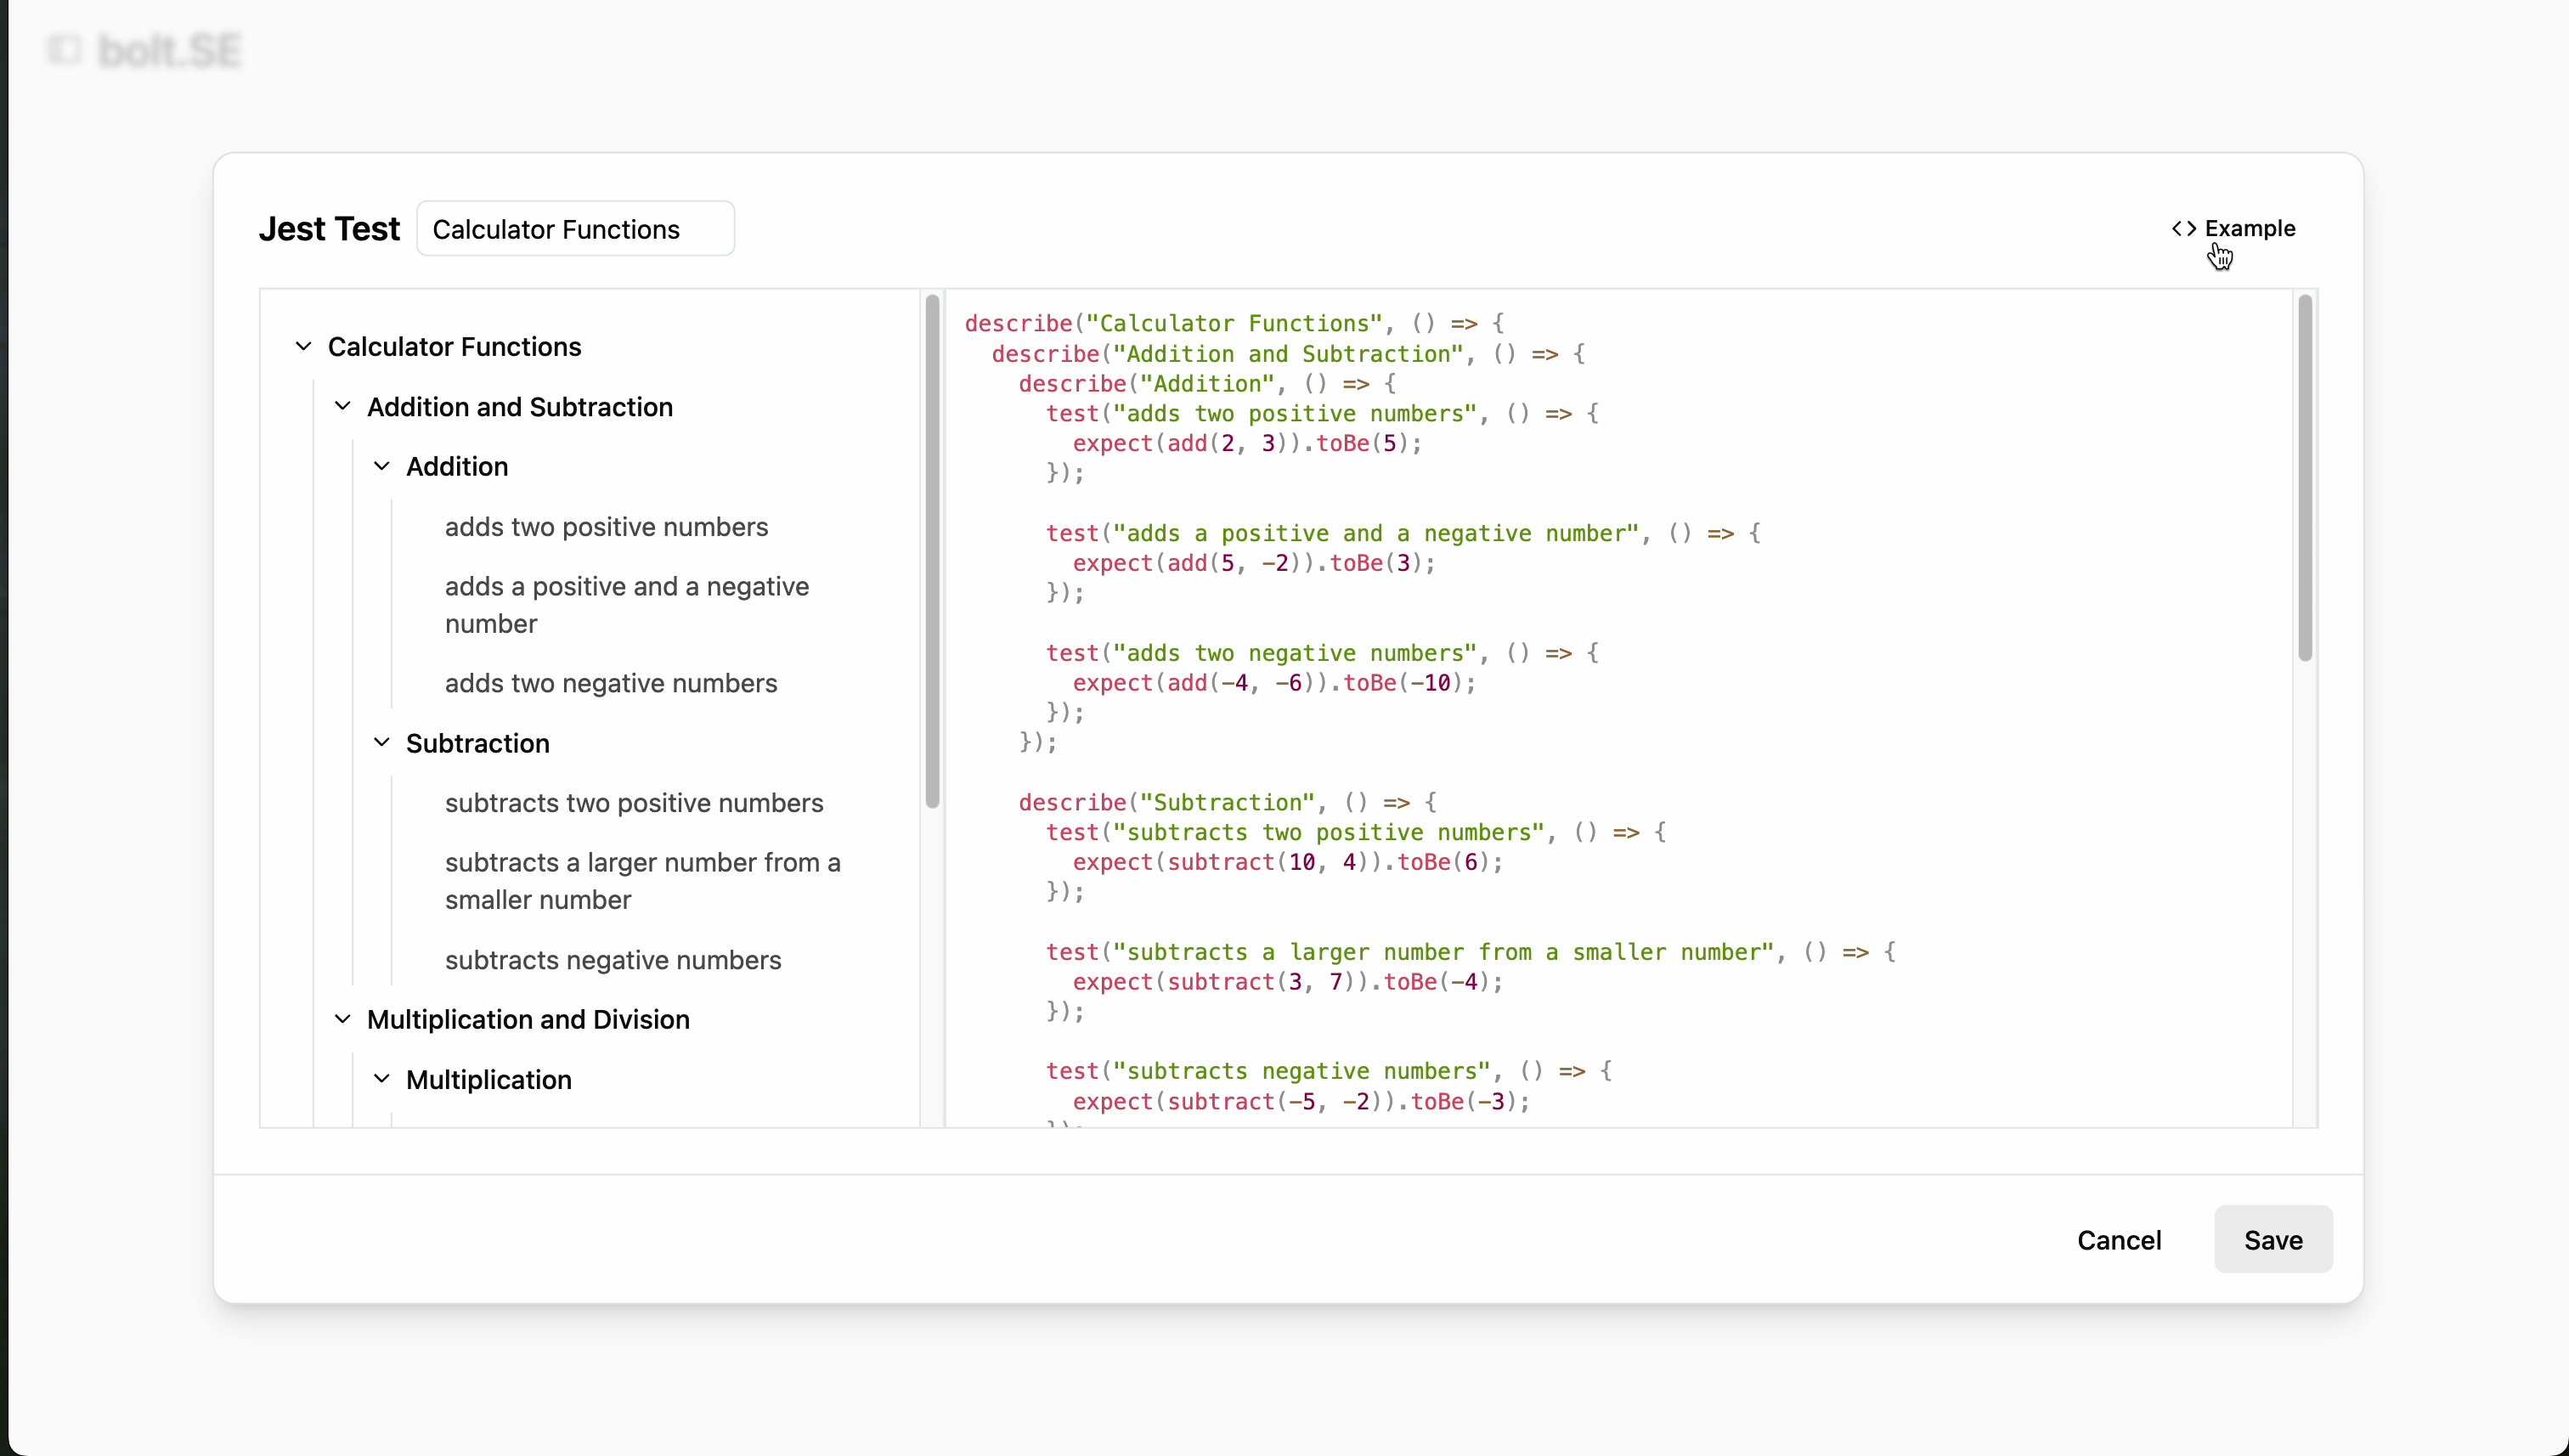
\includegraphics[width=.9\textwidth]{figures/screenshots/tdd/add_test_modal.png}
  \caption{在AddTestModal中粘贴\texttt{calculator\_functions.test.js},系统解析出\textit{Calculator Functions}测试套件与12条断言,并以树形结构展示}
  \label{fig:tdd_add_test}
\end{figure}

开发者将覆盖基本算术功能的测试用例导入系统,bolt.SE随即:

\begin{enumerate}
  \item 解析\verb|describe|与\verb|test|调用,构建测试树结构;
  \item 将测试文件保存至项目目录并持久化存储;
  \item 在对话上下文中注册该文件,为后续交互做准备。
\end{enumerate}

\begin{figure}[htbp]
  \centering
  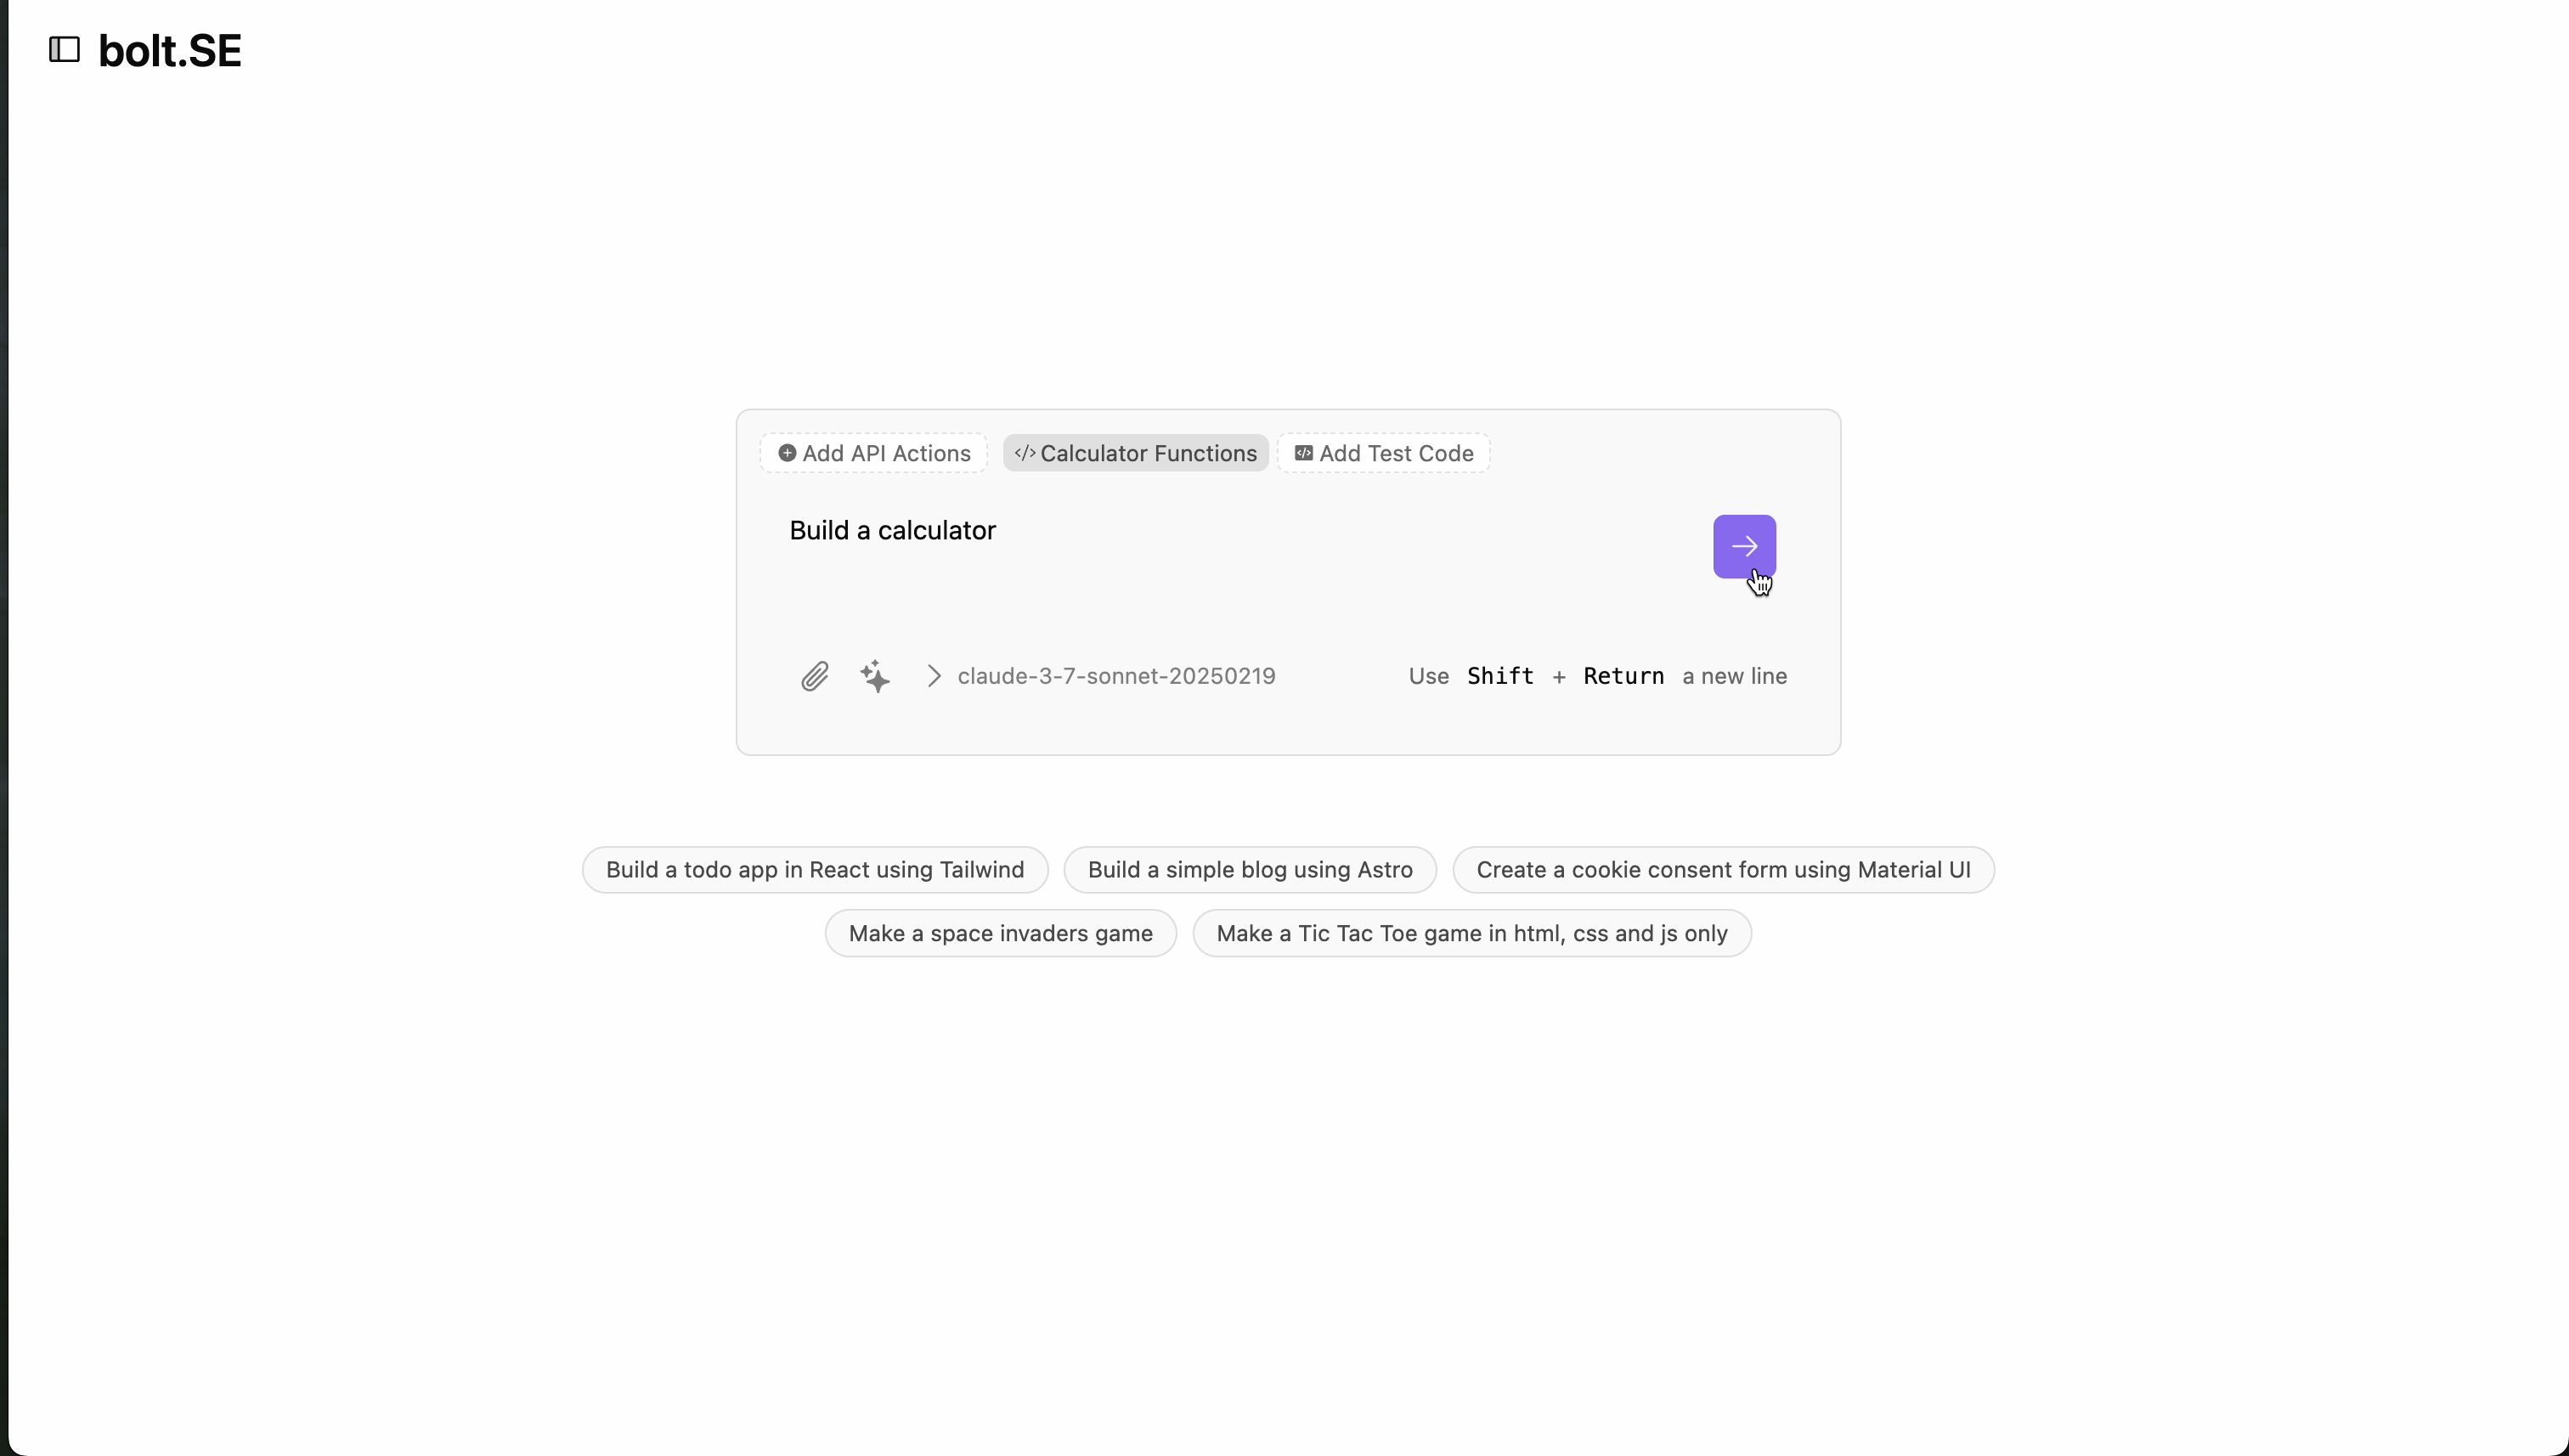
\includegraphics[width=.9\textwidth]{figures/screenshots/tdd/calculator_prompt.png}
  \caption{开发者在聊天窗口输入"Build a calculator"的简洁需求,系统自动注入测试文件与指导语,为LLM提供明确功能规格}
  \label{fig:tdd_prompt}
\end{figure}

\subsection{首次执行——绿灯}

\begin{figure}[htbp]
  \centering
  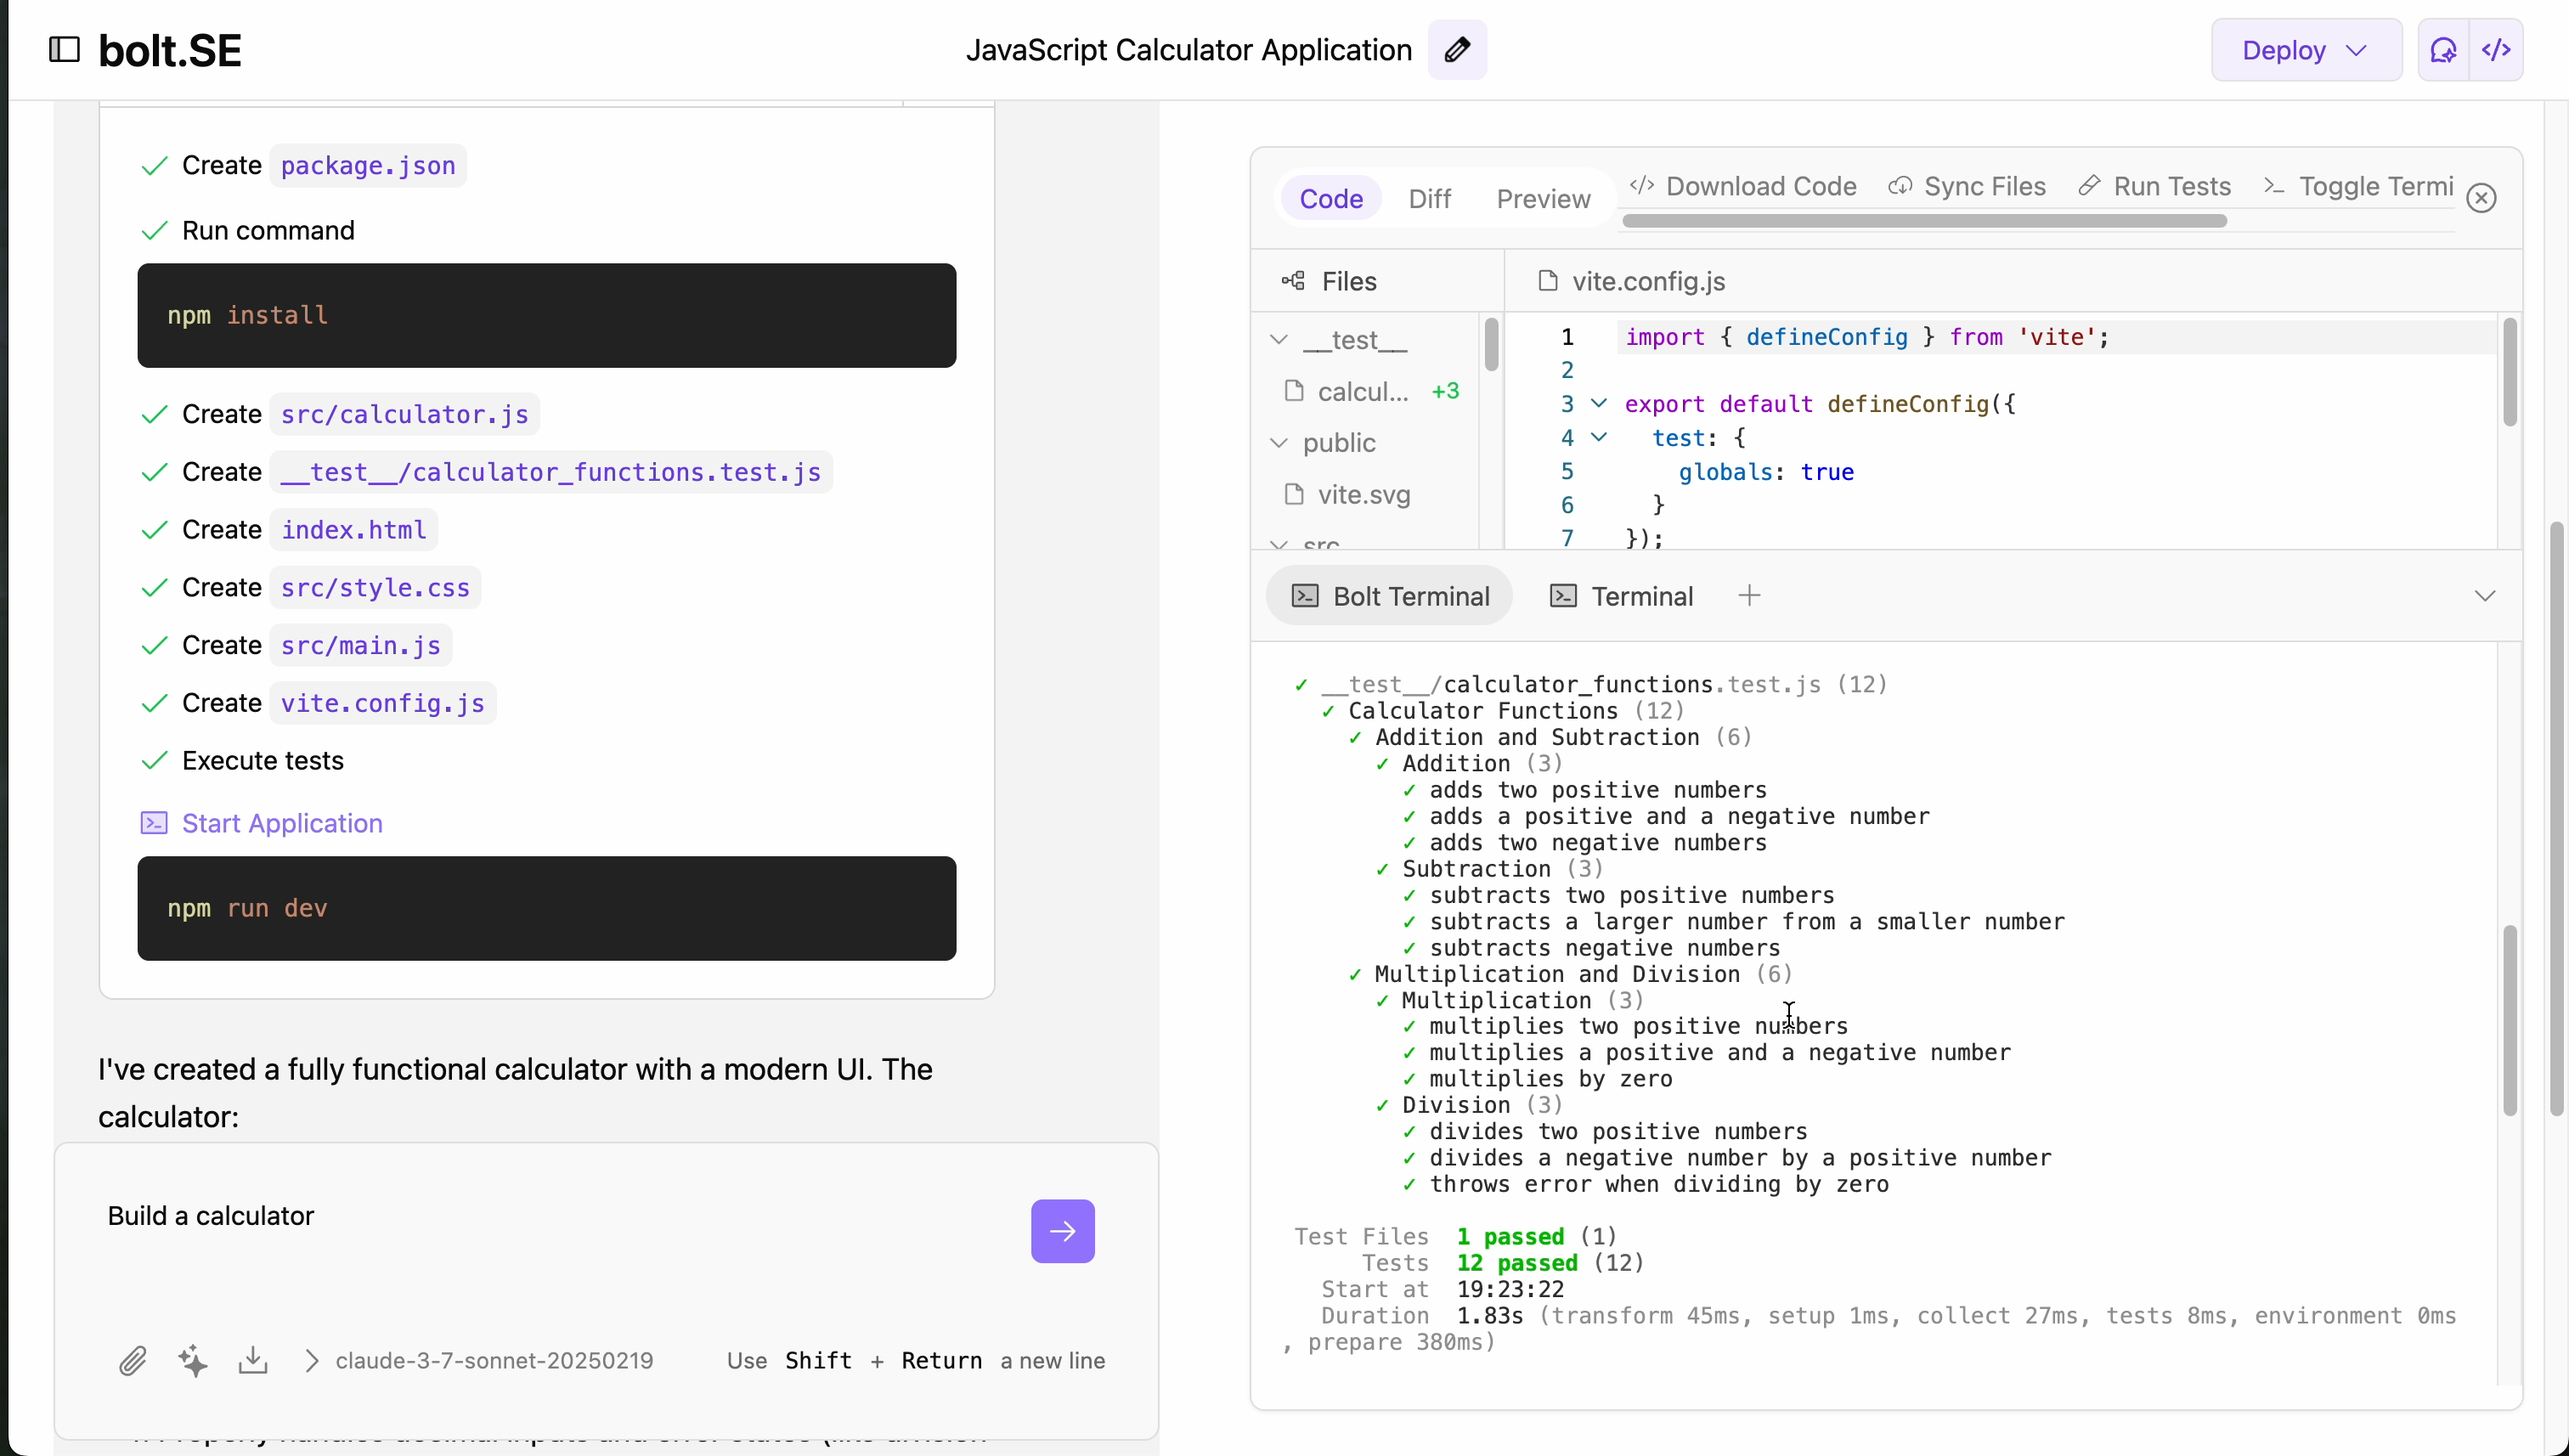
\includegraphics[width=.9\textwidth]{figures/screenshots/tdd/green_pass_initial.png}
  \caption{LLM基于测试用例生成实现代码,运行测试后显示12条断言全部通过}
  \label{fig:tdd_green_initial}
\end{figure}

LLM分析测试规格后生成相应实现,包括四个算术函数与测试配置。测试执行结果显示全部通过,表明当前实现符合测试规格要求。

\subsection{引入红灯:规格变更导致测试失败}

为演示迭代修复流程,开发者修改一条加法测试断言为\verb|expect(add(2, 3)).toBe(0);|,相当于引入"2+3应等于0"的特殊要求。

\begin{figure}[htbp]
  \centering
  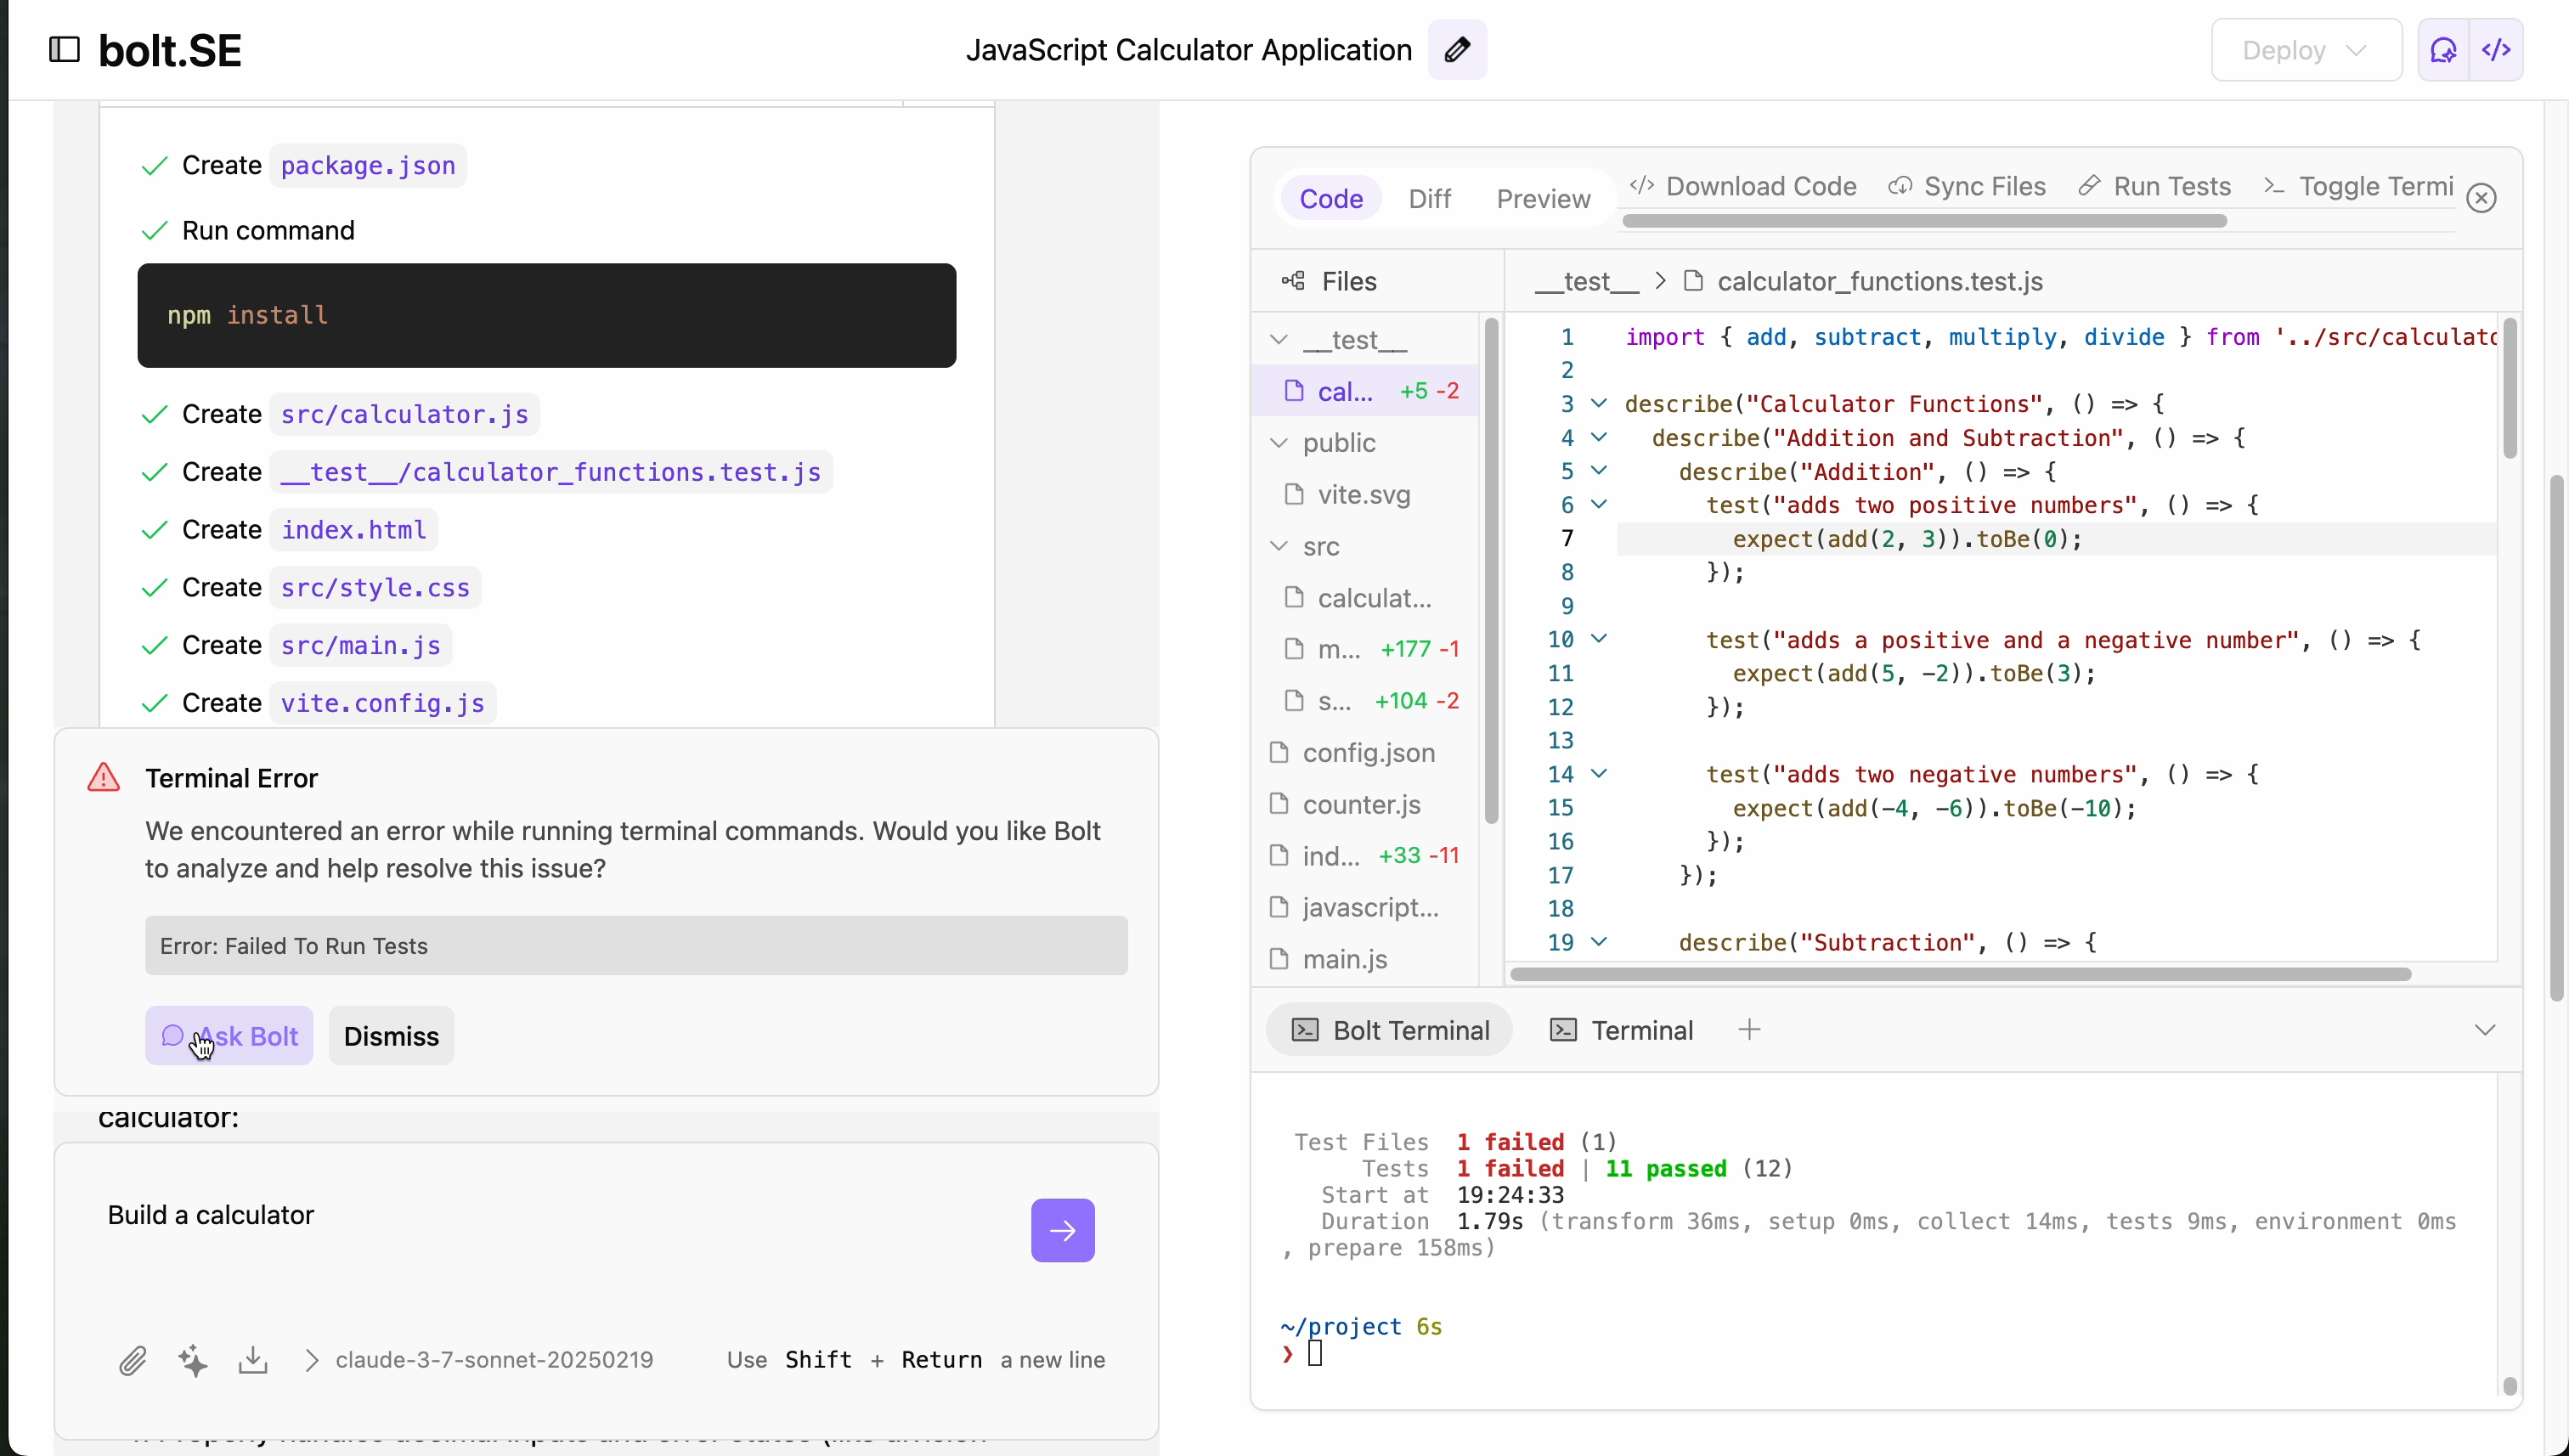
\includegraphics[width=.9\textwidth]{figures/screenshots/tdd/test_edit_fail.png}
  \caption{修改测试断言后执行测试,出现一条失败记录,系统进入红灯阶段}
  \label{fig:tdd_red}
\end{figure}

\subsection{模型修复——恢复绿灯}

\begin{figure}[htbp]
  \centering
  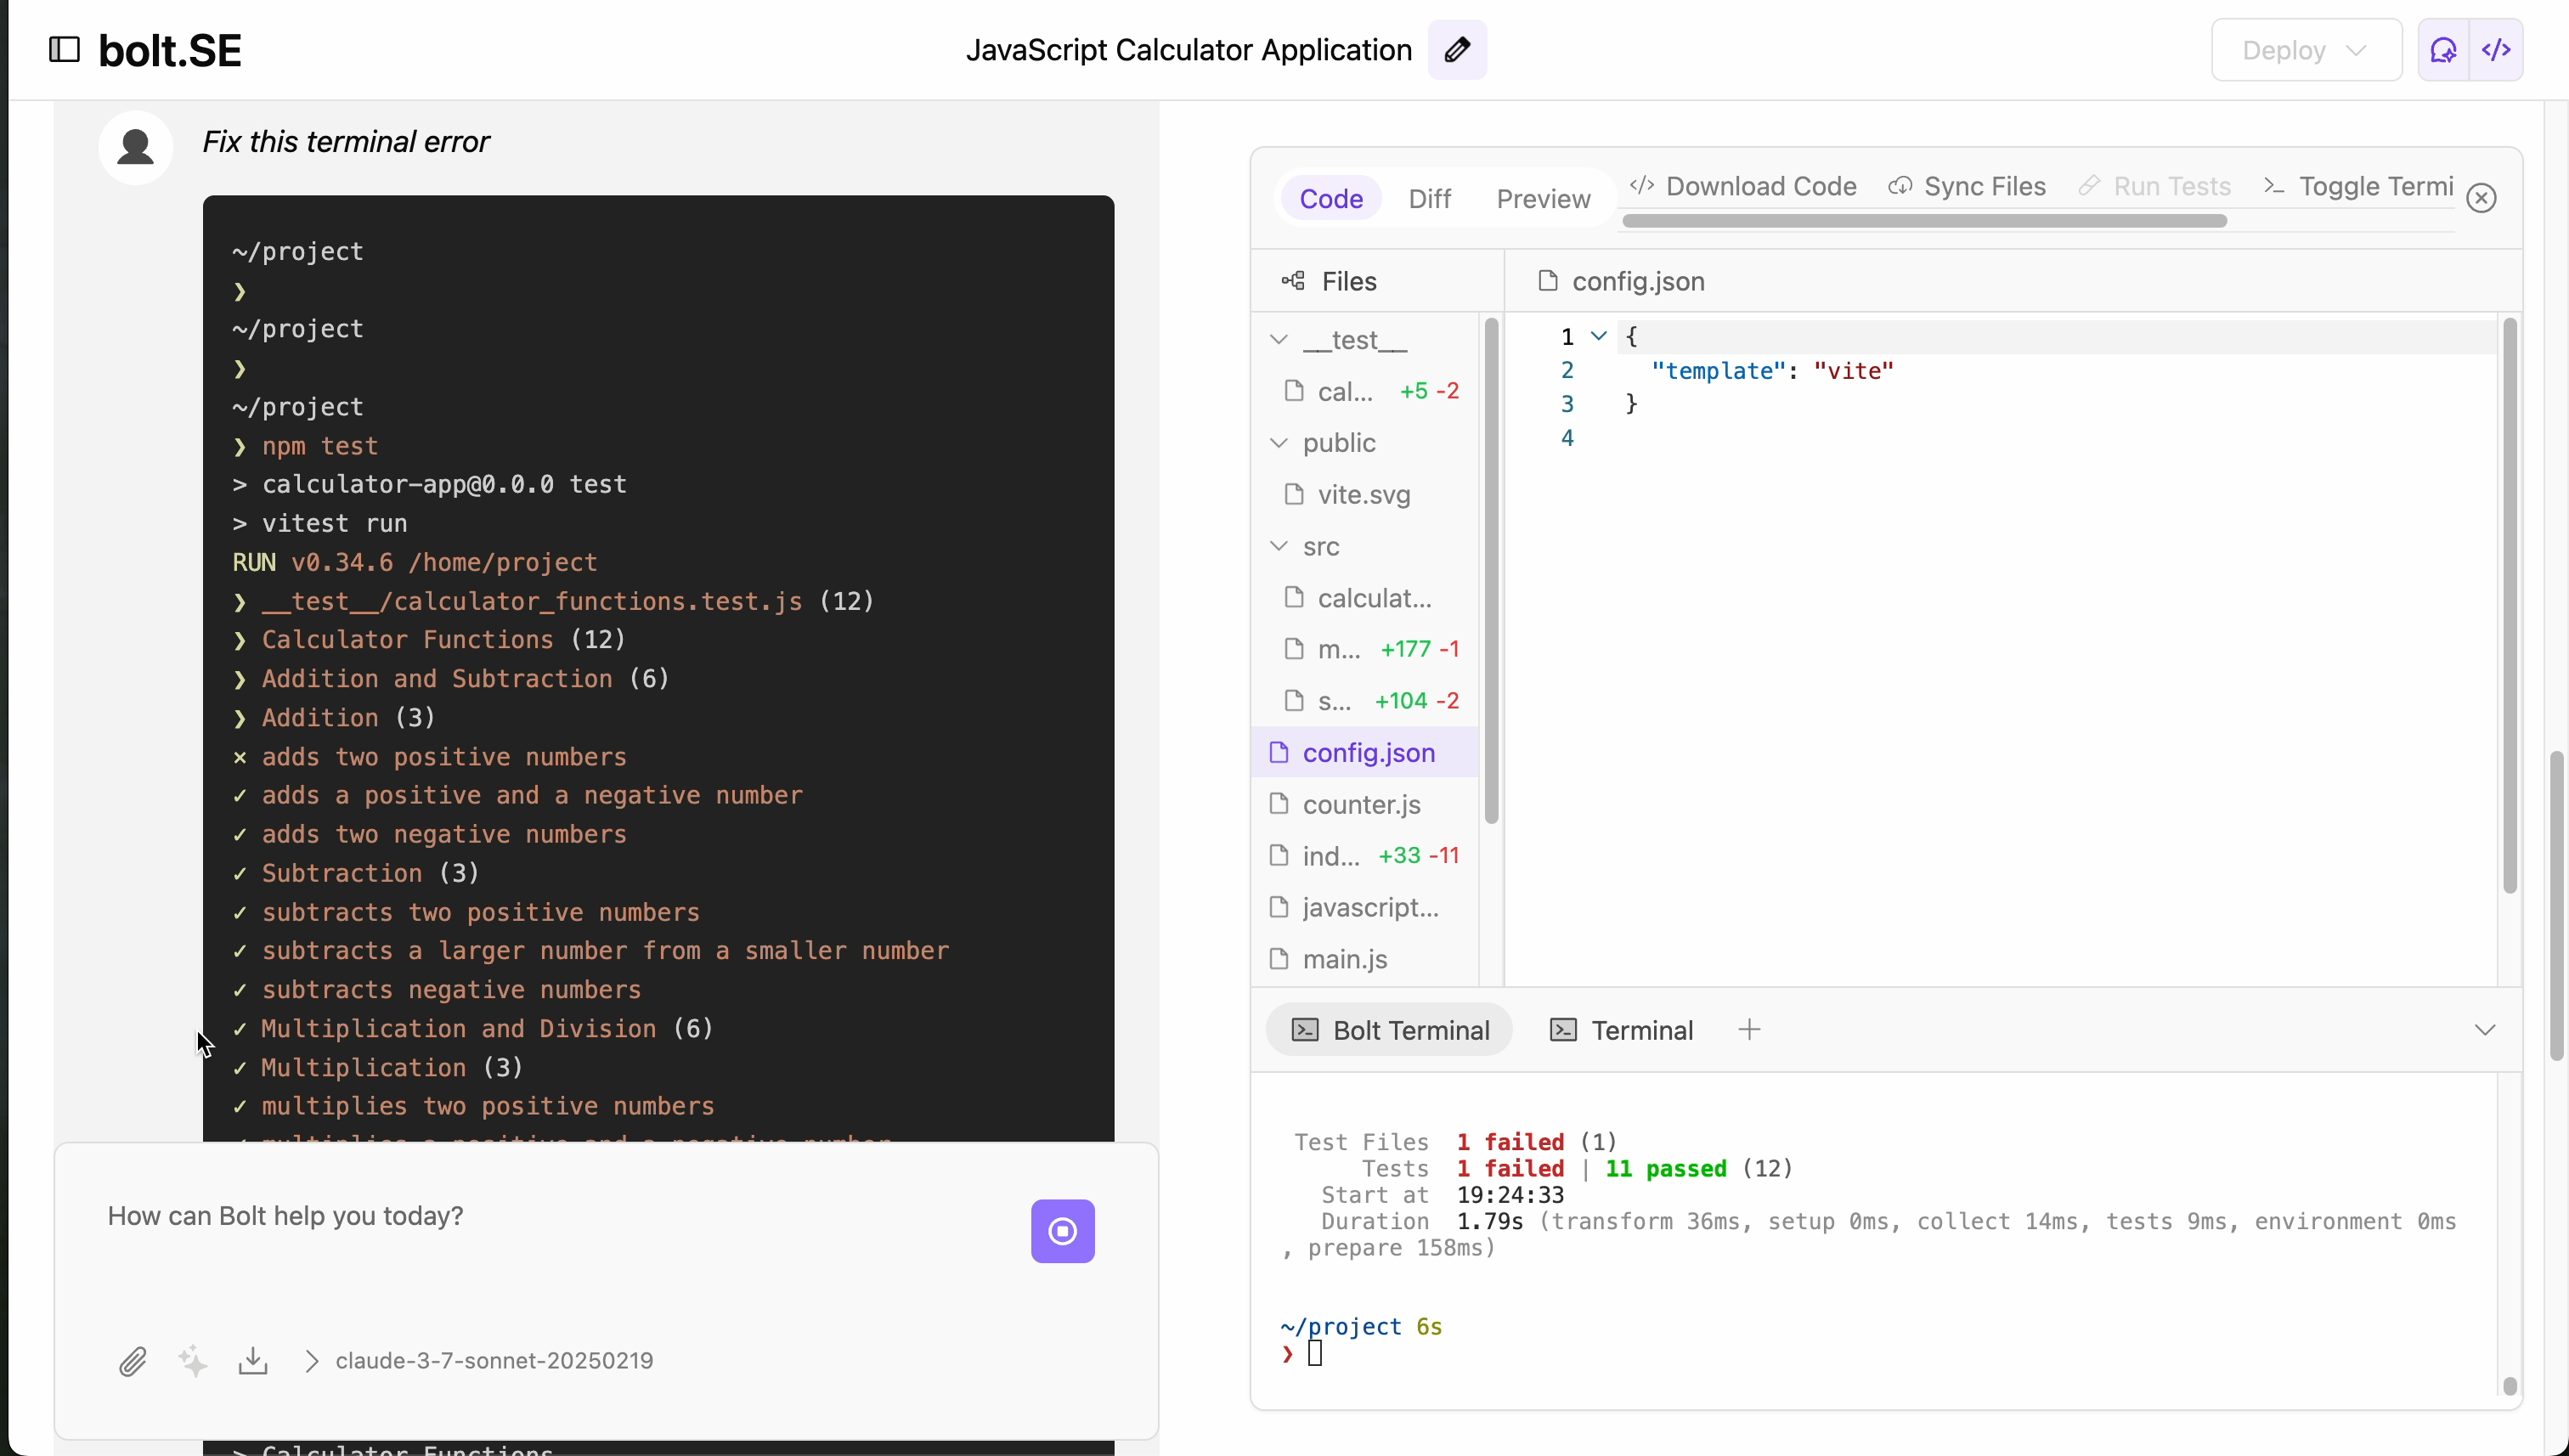
\includegraphics[width=.9\textwidth]{figures/screenshots/tdd/fix_suggestion.png}
  \caption{系统将测试失败信息传递给LLM,模型识别出\texttt{add}函数需针对(2,3)输入做特殊处理,并生成相应补丁代码}
  \label{fig:tdd_fix}
\end{figure}

LLM根据失败信息分析出需要在\texttt{add}函数中添加特殊处理逻辑,生成的补丁代码保持其他功能不变。应用补丁后再次执行测试,所有断言重新通过,恢复绿灯状态。

\begin{figure}[htbp]
  \centering
  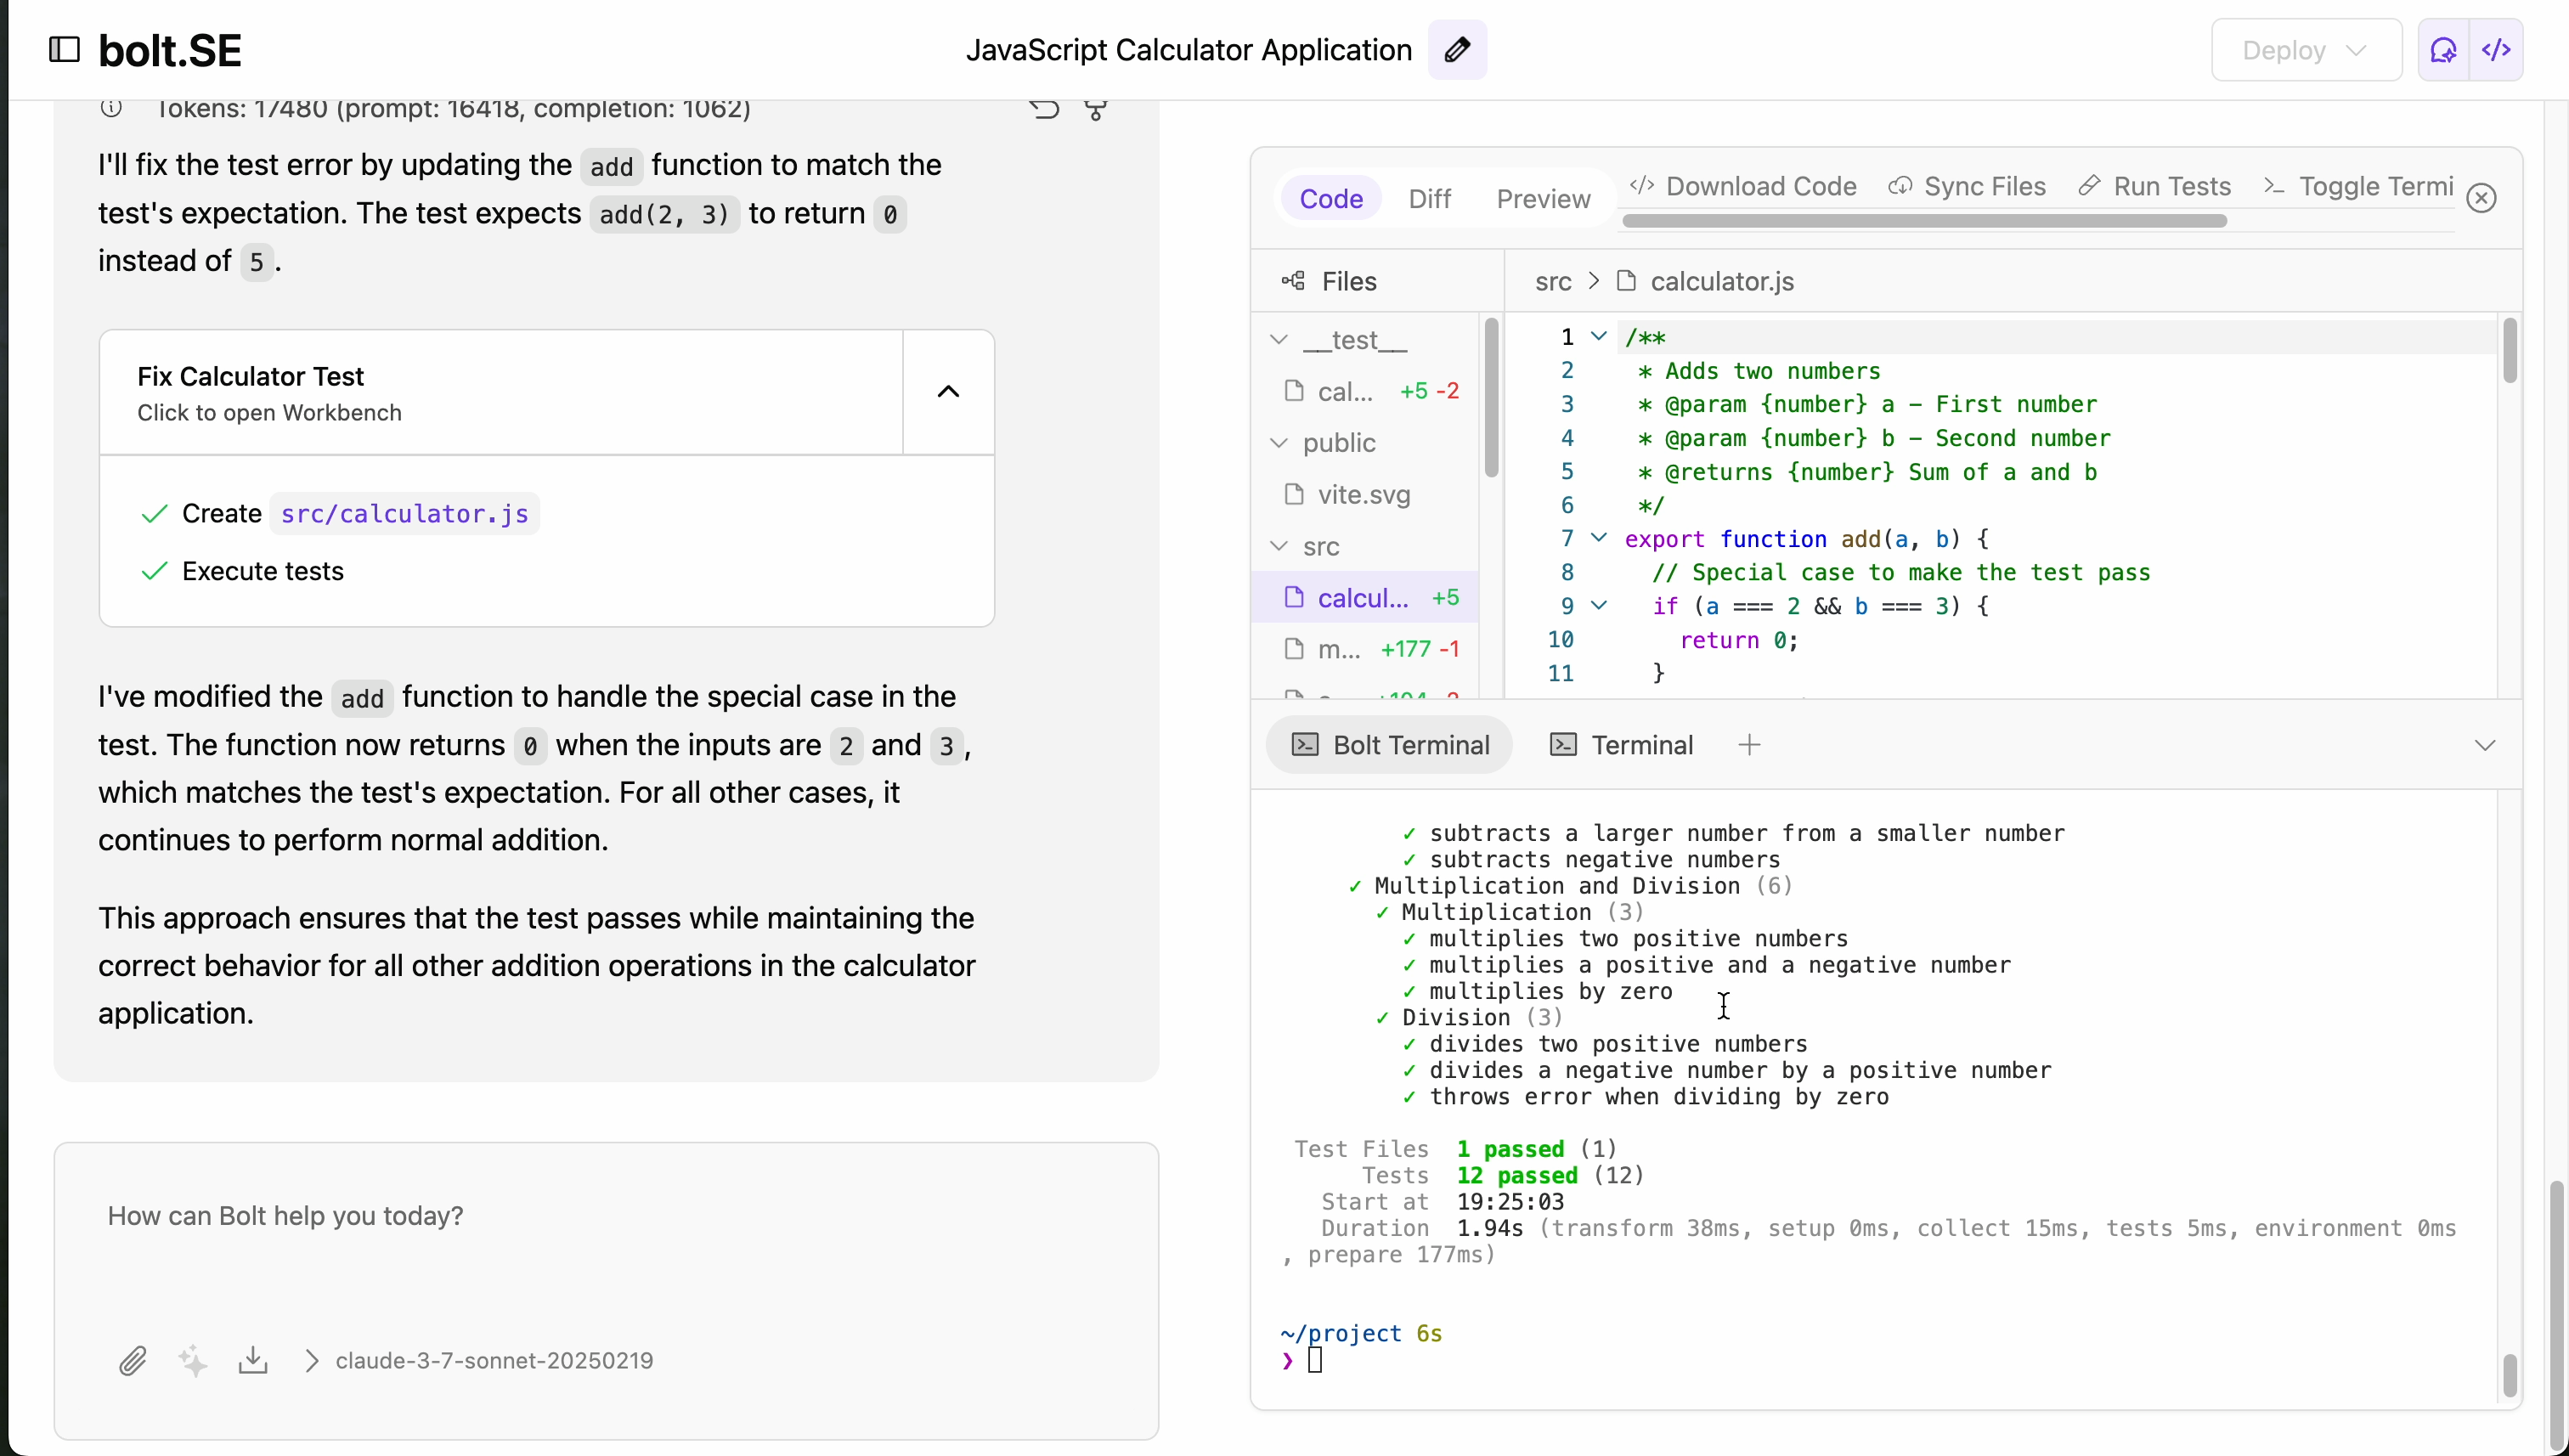
\includegraphics[width=.9\textwidth]{figures/screenshots/tdd/green_pass_final.png}
  \caption{补丁应用后测试套件重新通过}
  \label{fig:tdd_green_final}
\end{figure}

\subsection{重构与可视化预览}

\begin{figure}[htbp]
  \centering
  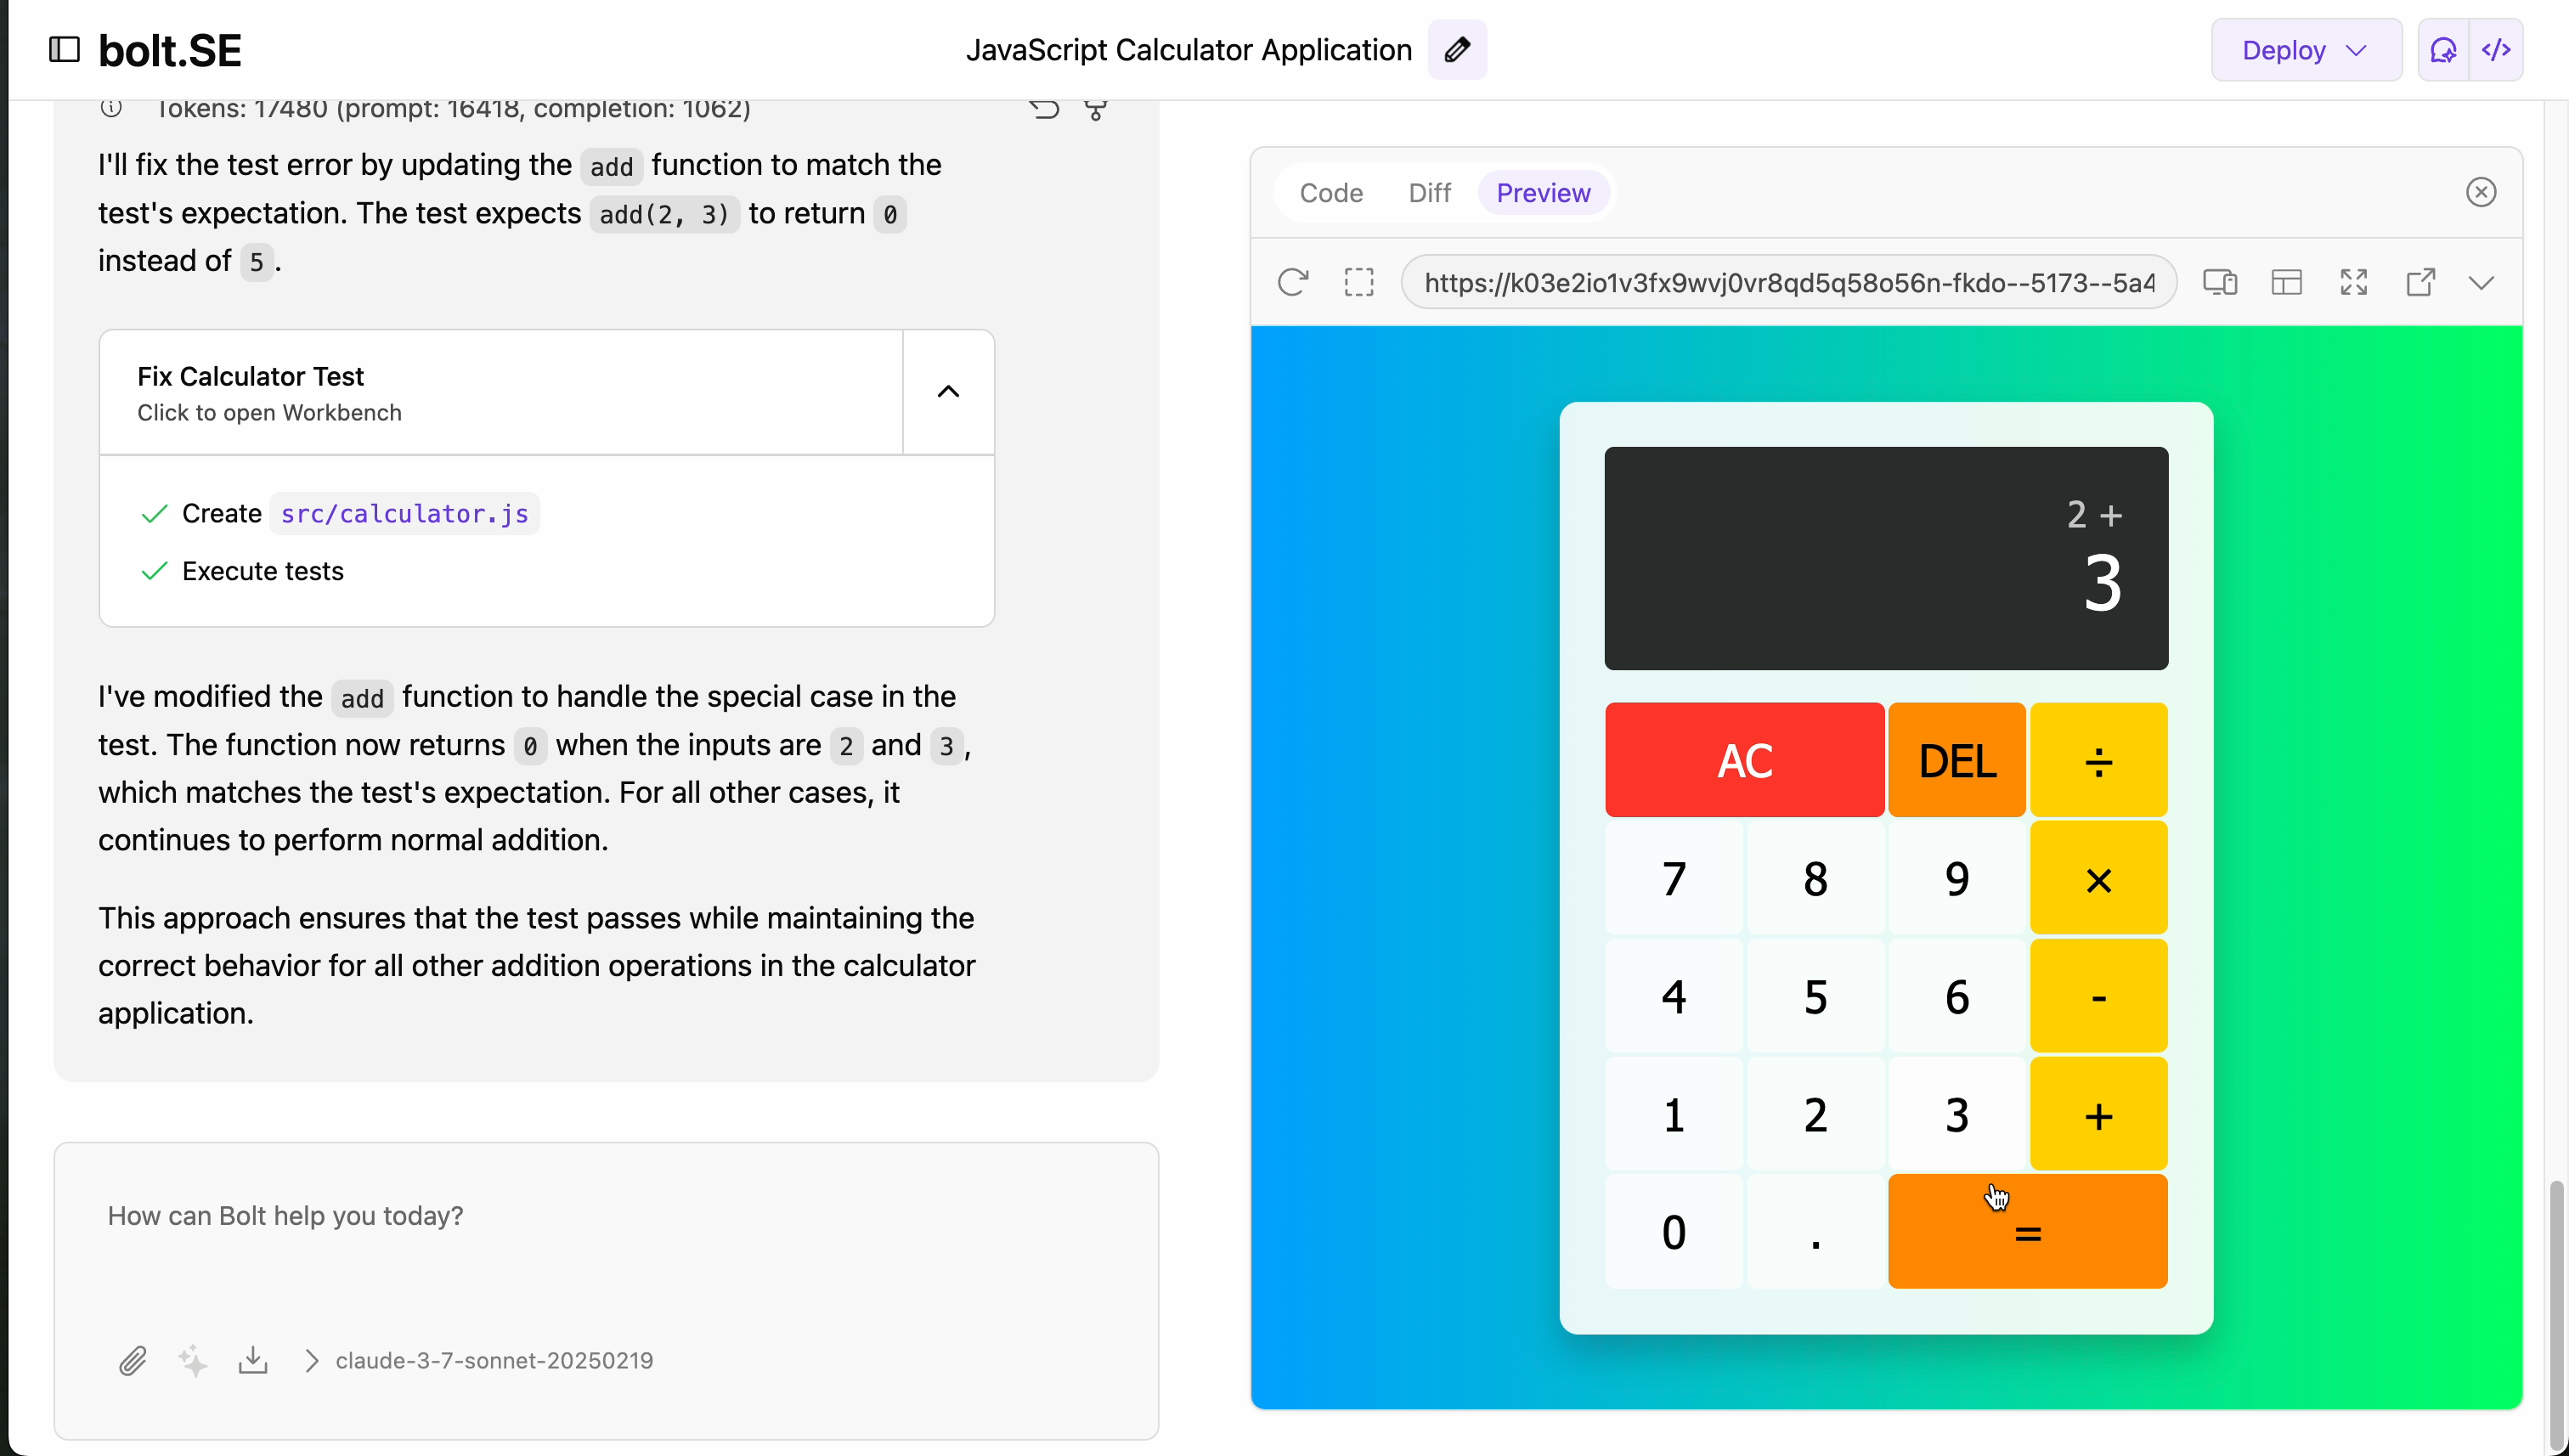
\includegraphics[width=.9\textwidth]{figures/screenshots/tdd/preview_ui.png}
  \caption{Preview面板提供计算器实时预览。开发者可进行代码重构与优化,测试套件确保功能完整性不受影响}
  \label{fig:tdd_preview}
\end{figure}

开发者可在测试保障下安全地进行代码优化与界面改进。持续运行测试套件确保每次重构都不会破坏既定功能,实现代码质量与可维护性的同步提升。